\documentclass[a4paper,12pt]{article}
\usepackage[left=2.54cm,top=2.54cm,right=2.54cm,includehead,nofoot]{geometry}
\usepackage{amsmath}
\usepackage{amssymb}
\usepackage[round]{natbib}	%for bibliography style natbib
\usepackage{setspace} %for double spacing
\usepackage{fancyhdr}
\usepackage{graphicx}	% for includegraphics
\usepackage{mathtools}
\usepackage{hyperref}	%for linking table of contents
\begin{document}
\pagestyle{headings}
\title{Turbulence as an accelerant of the homogenization process}
\author{Britta Hansen\\995260667}
\date{2013-04-15}
\maketitle
\markright{Britta Hansen 995260667}
\tableofcontents
\DeclareGraphicsExtensions{.jpg, .png}
\newcommand{\vecnorm}[1]{\left|\left|#1\right|\right|}
%%%%%%%%%%%%%%%%%%%%%%%%%%%%%%%%%%%%%%%%%%%%%%%%%%%%%%%%%%%%%%%%%%%%%%%%%%%%%%%%%%%%%%%%%%%%%%%%%%%%%%%%%%%%%%%%%%%%%%%%%%%%%%%%%%%%%%%%%%%%%%%%
\section{Introduction}

Mixing of fluids is often considered from a practical perspective in engineering. One might like to know how to improve their mixing device in order to blend the strongest polymers. Other applications include knowing how high to place a chimney so the fumes disperse well, or knowing where one should dispose of a toxic substance to minimize the impact on the surrounding wildlife. \doublespacing

The best mixers all have one thing in common: turbulence, defined as a flow whose trajectories are chaotic. But why does the presence of turbulence enhance homogeneity? Which properties of turbulent flows are most important for mixing? This paper intends to outline the reasons turbulence accelerates the mixing process as well as illustrate the presence and effect of turbulence with an example. 

Throughout, $v$ denotes the velocity of the bulk motion of the fluid and $\nu$ is the kinematic viscosity. Initial position vectors are represented by a capital $\vec{X}$ and the lower case $\vec{x}$ is the position vector at some time $t > 0$. Definitions are in bold face.
%%%%%%%%%%%%%%%%%%%%%%%%%%%%%%%%%%%%%%%%%%%%%%%%%%%%%%%%%%%%%%%%%%%%%%%%%%%%%%%%%%%%%%%%%%%%%%%%%%%%%%%%%%%%%%%%%%%%%%%%%%%%%%%%%%%%%%%%%%%%%%%%
\section{Why mixing?} 

Why is molecular diffusion insufficient to mix two substances? If D is molecular diffusivity (in units of $\frac{length^2}{time}$) and c is the concentration of the substance in question, then the diffusion equation is
\begin{align*}
\frac{\partial c}{\partial t} = D\frac{\partial^2 c}{\partial x^2}.
\end{align*} The general solution of which is proportional to the error function
\begin{align*}
c(x,t) \propto erf\left(\frac{x}{\sqrt{Dtn}}\right),
\end{align*} where n $\in \mathbb{R}$ depends on the dimension of the system (n is 2,4,6 for 1,2,3 dimensions respectively). So the distance over which the substance has diffused after time t is proportional to:
\begin{align}
\delta \propto \sqrt{Dt}.
\end{align}Recalling the shape of the square root function, this means that the distance grows quickly early on, and then slows down considerably for larger times. 

As a practical calculation, consider the diffusion of a lump of sugar in a cup of hot coffee. Using order-of-magnitude estimates:\\
$D_{sugar} = 0.5\times10^{-5}\text{ cm}^2s^{-1}$\citep[~p.1326]{hc09}\\
The coffee gets cold in about 30 minutes, or 1800 seconds, so from equation (1) the distance over which the sugar has diffused in 30 minutes is $\delta = 0.095\text{ cm}$. If the lump of sugar put in was a cubic centimetre in size, this means a volume of about $1.55\text{ cm}^3$ is occupied by sugar-water. But the cup of coffee has a radius of $3\text{ cm}$ and a height of $5\text{ cm}$. So the total volume of substance is $141\text{ cm}^3$, only 1.1\% of which is occupied by sugar water! It's clear that a better mixing mechanism, such as stirring, is required to sweeten a hot coffee.
%%%%%%%%%%%%%%%%%%%%%%%%%%%%%%%%%%%%%%%%%%%%%%%%%%%%%%%%%%%%%%%%%%%%%%%%%%%%%%%%%%%%%%%%%%%%%%%%%%%%%%%%%%%%%%%%%%%%%%%%%%%%%%%%%%%%%%%%%%%%%%%%
\section{Quantifying mixedness}

There are several different notions of how well-mixed a dynamical system is. Let ($X,\Sigma,\mu,T$) be a measure-preserving dynamical system, where $\Sigma$ is the sigma algebra, $\mu$ is the measure, and $T$ is a measure-preserving map representing time evolution, or flow. $A, B \in \Sigma$ are arbitrary measurable sets.
\\ \\
A system is \textbf{strong measure theoretic mixing} (SMTM from here on) if for any two measureable sets, $A$ and $B$, as time goes to infinity these two sets necessarily intersect. 
\begin{align*}
\lim_{n \to \infty} \mu(A \cap T^{-n}B) = \mu(A)\mu(B)
\end{align*} SMTM is the considered the best form of mixing possible, and so can be seen as the ultimate end goal \citep[~p.119]{o81}.
\\ \\
A system is \textbf{strong topological mixing} if any two open sets will eventually intersect. Clearly SMTM implies STM because all open sets are measurable.
\\ \\
A system is \textbf{weak mixing} if, similar to strong mixing, any two measurable sets intersect. 
\begin{align*}
\lim_{n \to \infty} \frac{1}{n} \sum^n_{k=0} \left(\mu(A \cap T^{-n}B) - \mu(A)\mu(B)\right) = 0
\end{align*} The difference between this and SMTM is that the notion of convergence of the limit is weaker here than in SMTM. In weak mixing the convergence is specifically Ces{\'a}ro type, which will not be ellaborated on here, except for the fact that Ces{\'a}ro convergence is weaker than regular convergence.
\\ \\
A point $\vec{x}$ is called \textbf{wandering} if there exists a neighbourhood $U$ of $\vec{x}$ and a time $t'$ such that $\forall t>t'$, the point never returns to $U$. If the set of wandering points has positive measure, then the system is dissipative. Homoclinic points are non-wandering. The existence of non-wandering points is necessary for the aperiodic long-term behaviour characteristic of chaos. For instance, most of the points on an attractor of dimension smaller than the phase space must be non-wandering, for they never leave the attractor and yet never return to precisely the same position, so they come arbitrarily close to their previous positions.
\\ \\
A system is \textbf{ergodic} if its time average is the same as its phase space average:
\begin{align*}
\forall \text{ A,B } \in \Sigma, \text{ both with positive measure, } \exists \text{ n}>0 \text{ such that } \mu(T^{-n}A\cap B) > 0
\end{align*} The implications of these different definitions of mixing can be seen from this image:\\
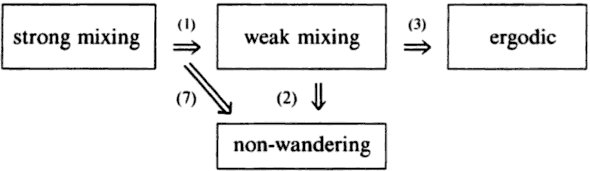
\includegraphics[scale=0.6,natwidth=590, natheight=171]{topologicalhierarchy} \\ \tiny{\citep[~p.75]{v93}} \\ \normalsize
The converse to any of these arrows is false so none of the above definitions are equivalent, and non-wandering does not imply ergodic \citep[Proposition 4.4]{v93}. The product of a weakly mixing and strongly mixing flow is ergodic \citep[Proposition 4.17]{v93}
%%%%%%%%%%%%%%%%%%%%%%%%%%%%%%%%%%%%%%%%%%%%%%%%%%%%%%%%%%%%%%%%%%%%%%%%%%%%%%%%%%%%%%%%%%%%%%%%%%%%%%%%%%%%%%%%%%%%%%%%%%%%%%%%%%%%%%%%%%%%%%%%
\section{Mechanisms by which turbulence aids mixing}

Disregarding flows involving chemical reactions and time-irreversible systems, generally it is believed that flows are \textbf{homeomorphic} (continuous bijections with continuous inverses). Continuity is obvious since we don't believe particles can disappear and reappear, and thus their positions (governed by the flow) must be continuous. Bijectivity is required if we don't want 2 particles occupying precisely the same place in space, nor do we want particles merging or splitting apart. Continuous inverses are implied by the time-reversibility. 

If the particle velocity field is continuous as well then the flow is \textbf{1-diffeomorphic}, since the velocity is the derivative of the flow. This can be used to take advantage of the very nice properties of diffeomorphisms; they preserve almost any topological structure imagineable. 

One important property of homeomorphisms is that they preserve connectedness \citep[thm 23.5]{m00}. Homeomorphic flows also map boundary points to boundary points \citep[Problem 2.2.2. Solution included in the appendix]{o81}. 

Now supposing a flow is diffeomorphic, then in order to preserve the topology of blobs of fluid to be mixed, the blobs must become highly distorted. Recalling the above definitions of mixing, the two different fluids must be present no matter how close we zoom in. This gives an extreme perception of just how distorted we want to make the blobs! Let's see how this is possible.

\subsection{Stretching, folding, and cutting}

Just how well-mixed can we make fluids simply by folding, stretching, and cutting the blobs? We're already familiar with the baker's map, which involves all three actions of stretching, folding, and cutting. The presence of a baker's map implies SMTM, in the sense that a flow is SMTM in a region R if and only if there exists a homeomorphism of R to a square under which the flow becomes a baker's transformation \citep[p.~119]{o81}. So baker's maps yield the best form of mixing, and we'd like to incorporate them, or closely mimic them, in our mixing apparati.

However, since continuous flows preserve connectedness, they therefore don't allow for cutting. The baker's map is thus unrealistic. A similar map without cutting is the horseshoe map. The procedure for its construction is as follows: stretch out the square, fold it over next to itself, and then repeat with the highlighted square in the third image here:\\
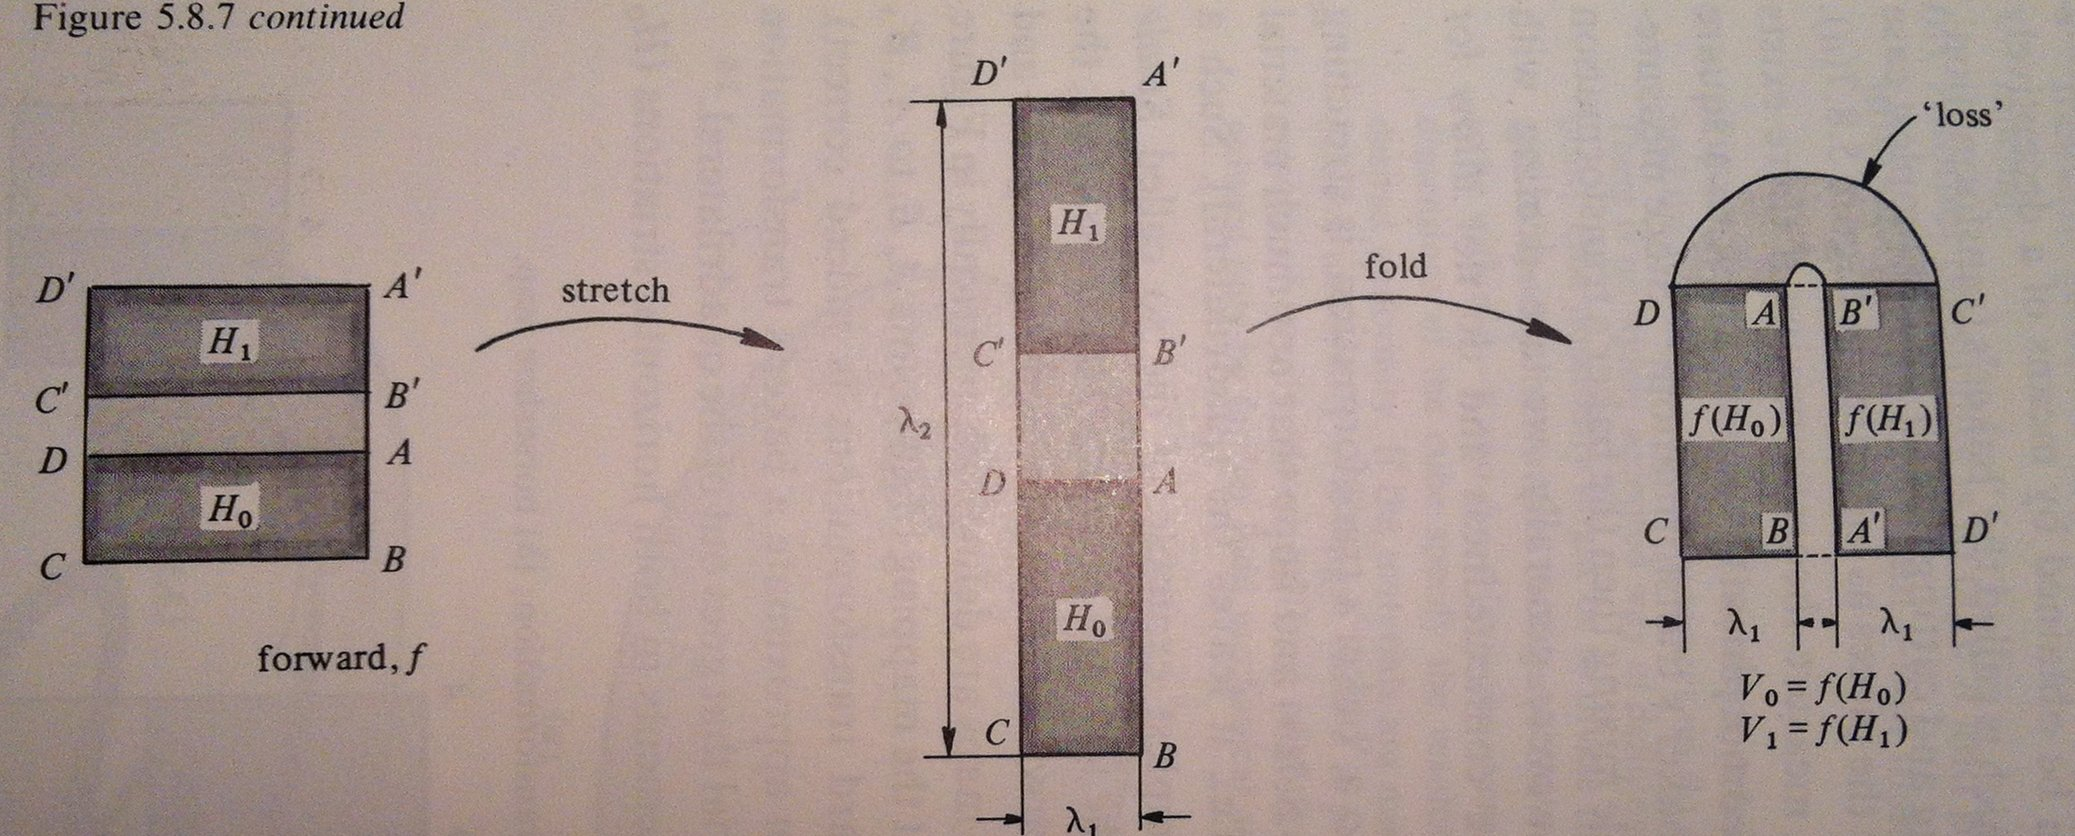
\includegraphics[scale=0.22,natwidth=2075,natheight=836]{horseshoe}\\ \tiny{\citep[Fig. 5.8.7]{o81}} \\ \normalsize
Although similar to the baker's map it does not contain the cutting step and so it arises frequently in commercial mixing processes. The lack of cutting causes the horseshoe map to miss out on SMTM and so systems involving horseshoe maps don't mix as well as those with baker's maps. The reason for this is apparent when we examine the steps of the horseshoe map: note that the middle portion of the first step is lost in the third step. Normally in the baker's map we would cut that piece off and glue it back to the square so that it is included in future mixing. However, by disregarding it (since we can't cut) that portion essentially goes unmixed in the transformation. The horseshoe map thus leaves many portions of material unmixed, and we need to rely on other mixing mechanisms such as molecular diffusion to improve the homogenization of these parts. 

A \textbf{homoclinic tangle} is a homoclinic point in which the stable and unstable manifolds intersect each other an infinite number of times. Their presence is often indicative (or even part of the definition) of chaos. The horseshoe map contains a homoclinic tangle, and its presence is always an indication of chaos.

The amount by which material elements are stretching is commonly quantified by the \textbf{Liapunov exponents}
\begin{align}
\sigma _i (\vec{X})= \lim_{\substack{t \to \infty\\ \vecnorm{d\vec{X}} \to 0}}\left(\frac{1}{t}\ln\left[\frac{\vecnorm{d\vec{x}}}{\vecnorm{d\vec{X}}}\right]\right),
\end{align} where $d\vec{x}$ and $d\vec{X}$ are displacements in the position and intial position vectors respectively. An important question to consider is ``When does the limit in (2) exist?''. In 1968 Oseledec showed that there is a set of initial conditions called \textbf{regular points} for which the limit exists \citep{o68}. For volume-preserving flows the regular points have full Lesbegue measure. This raises an interesting point: when we speak of the set of admissible initial conditions, we're not necessarily speaking of the entire space itself, for some of the points in the phase space may not yield well-defined quantifications of the flow geometry. Liapunov exponents are basically the long time average of the specific rate of stretching.

Also noteworthy is that Batchelor created a rate of `local' stretching for infinitesimal elements and thus also created a local Lyapunov exponent. However, there is no theorem (as of 1995) that the limit for this local Lyapunov exponent ever exists \citep[~p.295]{tk95}. 
%%%%%%%%%%%%%%%%%%%%%%%%%%%%%%%%%%%%%%%%%%%%%%%%%%%%%%%%%%%%%%%%%%%%%%%%%%%%%%%%%%%%%%%%%%%%%%%%%%%%%%%%%%%%%%%%%%%%%%%%%%%%%%%%%%%%%%%%%%%%%%%%

\subsection{Cascading energy} 

An idea proposed by Kolmogorov is that friction only acts on the smallest scales to dissipate energy. In order for conservation of energy to hold, energy must thus be coming from the larger scales through kinematic processes, such as large eddies and vorticies. The cost in energy is an important factor to consider for practical purposes of mixing: it would take a lot more energy to mix a high viscosity substance than a low viscosity one. 

Kolmogorov constructed length and velocity scales to describe the smallest eddies, and thus also a timescale. Let $\epsilon$ be the rate of kinetic energy dissipation per unit mass (units of $\frac{length^2}{time^3}$). By the model of cascading energy, the kinetic energy is dissipating from the bulk motions of the fluid and is being transported into the smallest scales, only to be dissipated as heat. Using dimensional analysis to obtain the rate of dissipation per unit mass  it is found that 
\begin{align}
\epsilon = \frac{v^3}{L}.
\end{align}Let the Kolmogorov length and velocity scales be
\begin{align}
\ell &= \left(\frac{\nu^3}{\epsilon}\right)^{1/4}\\
u_{\ell} &= (\nu\epsilon)^{1/4}
\end{align} respectively \citep[~p.47]{h99}. Then the time scale obtained by dimensional analysis is
\begin{align}
\tau &= \frac{\ell}{u_{\ell}}\\
&= \sqrt{\frac{\nu}{\epsilon}}
\end{align} The idea is that at this length scale, viscosity dominates, and so it's the smallest length scale for energy transfer in turbulent systems. We will return to these length scales when we look at the Reynolds number. The scales of the large eddies are set by the geometry and speed of the stirring mechanism, while the cut-off scales of the small eddies are determined by the action of viscosity. $\ell << L$ means there is a range of intermediate sizes of eddies, allowing for the self-similar patterns often observed of chaotic systems.

The derivations of these scales rely on several assumptions. For one, it's assumed that the rate at which energy is transferred from one scale to another is equal to the rate of kinetic energy dissipation. Also, it is assumed that only viscosity plays a role in dissipating this energy into heat, and finally Kolmogorov believed that at small length scales the system is statistically isotropic.

So how reasonable are these assumptions? It is known experimentally that ``the mixing time depends linearly on the initial size of the blob to be mixed" \citep[~p.4]{vcc99}, yet Kolmogorov's theory would give us a mixing time proportional to the initial length to the $\frac{2}{3}$-power. It is also known that energy can in fact be transferred from small scales back to large scales in a process called `backscatter' \citep[~p.606]{cgm95}. 
%%%%%%%%%%%%%%%%%%%%%%%%%%%%%%%%%%%%%%%%%%%%%%%%%%%%%%%%%%%%%%%%%%%%%%%%%%%%%%%%%%%%%%%%%%%%%%%%%%%%%%%%%%%%%%%%%%%%%%%%%%%%%%%%%%%%%%%%%%%%%%%%
\subsection{KAM theory} 

A theory named after it's pioneers Kolmogorov, Arnold, and Moser. In essence, the theory states that most trajectories of a nearly integrable Hamiltonian system (nearly integrable in the sense that it's a perturbation of an integrable Hamiltonian system) remain quasi-periodic. So for an integrable Hamiltonian system, the angular variables precess around N-dimensional tori with a particular angular frequency. Although the unperturbed system has tori formed by both periodic and quasi-periodic solutions, the quasi-periodic ones are more stable in the sense that all but finitely many of the periodic solutions are destroyed by the perturbation. For an introduction to KAM theory see \cite{w08}. 

These KAM tori offer significant results for mixing: since the tori are invariant, no trajectories can intersect them, and thus they split the phase space into inaccessible regions. A particle which begins on the outside of a KAM torus will forever remain outside. As a result, no flow containing a KAM torus can ever be SMTM, for any measurable set exterior to the KAM torus can never intersect the torus. For practical purposes, if a mixing procedure produces KAM tori one may attempt to reduce the size of the tori until they are on the scale of molecular diffusion, and then let diffusion provide the rest of the mixing.
%%%%%%%%%%%%%%%%%%%%%%%%%%%%%%%%%%%%%%%%%%%%%%%%%%%%%%%%%%%%%%%%%%%%%%%%%%%%%%%%%%%%%%%%%%%%%%%%%%%%%%%%%%%%%%%%%%%%%%%%%%%%%%%%%%%%%%%%%%%%%%%%
\section{Dimensionless numbers and their impact on homogeneity} 

Pervasive throughout fluid mechanics are dimensionless numbers. They provide an easy check of the relevance and importance of certain factors in achieving a particular outcome. Although useful, dimensionless numbers are by no means deterministic: given any dimensionless numbers one can construct uncountably many more simply by taking powers and products of them, but how do we know which are the `correct' ones to describe the outcome we're looking for? It's not clear since they are never derived from first principles but are instead an outcome of dimensional analysis. Also, many dimensionless numbers require grossly simplifying assumptions be made about the system, such as ``the viscosity is so high the inertial terms basically vanish" or ``suppose surface tension is negligible". While these assumptions are fine in many cases they must be applied with caution; dimensionless numbers which are derived by these assumptions must not be applied to systems in which the assumptions no longer hold.

Here they are separated into intrinsic and extrinsic numbers. Intrinsic numbers depend only on the properties of the fluids at hand (viscosity for example). Extrinsic numbers depend on the geometry and boundary conditions of the flow (as in length scales and periodicity). The relevance of separating the two is that intrinsic numbers can tell us if a certain outcome (perhaps SMTM) is possible with a particular fluid or not, whereas extrinsic numbers might tell us how to modify our mixer in order to improve the mixing. 

All of the analyses on these dimensionless numbers will promote Kolmogorov's theory of cascading energy. Although this theory is known to be incorrect, experimentally it's not far off and offers plausible explanations of turbulent flows. As such, it's the only analysis I'm capable of giving.
%%%%%%%%%%%%%%%%%%%%%%%%%%%%%%%%%%%%%%%%%%%%%%%%%%%%%%%%%%%%%%%%%%%%%%%%%%%%%%%%%%%%%%%%%%%%%%%%%%%%%%%%%%%%%%%%%%%%%%%%%%%%%%%%%%%%%%%%%%%%%%%%
\subsection{Reynolds number (extrinsic)}  

Consider the Reynolds number $R = \frac{vL}{\nu}$, where $L$ is the characteristic length scale. It is the ratio of the viscous time scale and the convective time scale and thus describes which is causing change at a faster rate, inertia or viscous stresses. 

Recalling equation (6) from the Kolmogorov scales, it is found that the ratio of small to large length scales is given by 
\begin{align}
\frac{\ell}{L} = R_e^{-3/4}
\end{align} It has been shown repeatedly that high Reynolds number is a necessary condition to sustain turbulence \citep[p.~61]{dc99}. From the theory of cascading energy, viscosity is only important on small scales, thus low Reynolds numbers imply high viscosities and lots of energy lost due to friction, therefore low Reynolds number flows tend to cost more energy to mix. 

Now we can better understand how stretching and folding help the mixing process, at least within the paradigm of cascading energy. Apart from causing initial conditions to separate as was seen with the Liapunov exponent, the act of folding material lines is creating smaller and smaller length scales. As $\frac{\ell}{L}$ decreases, kinetic energy is able to dissipate at smaller and smaller scales and the Reynolds number increases. Also at small scales, the turnover time of the smallest eddies $\tau$ is very small, so the eddies change rapidly.
%%%%%%%%%%%%%%%%%%%%%%%%%%%%%%%%%%%%%%%%%%%%%%%%%%%%%%%%%%%%%%%%%%%%%%%%%%%%%%%%%%%%%%%%%%%%%%%%%%%%%%%%%%%%%%%%%%%%%%%%%%%%%%%%%%%%%%%%%%%%%%%%
\subsection{Richardson number (extrinsic)} 

Let $h$ be a characteristic vertical length scale. The Richardson number is then the ratio of graviational potential energy to kinetic energy
\begin{align*}
R_i = \frac{gh}{v^2}.
\end{align*} If this number becomes much larger than unity, buoyancy becomes important. If this is the case, the restoring buoyant forces cause stratification of the fluids, in which they tend to align themselves in smooth, horizontal layers for which the surfaces of these layers are minimal energy configurations. In this case there is insufficient kinetic energy to overcome this stratification and the fluids will not homogenize. 
%%%%%%%%%%%%%%%%%%%%%%%%%%%%%%%%%%%%%%%%%%%%%%%%%%%%%%%%%%%%%%%%%%%%%%%%%%%%%%%%%%%%%%%%%%%%%%%%%%%%%%%%%%%%%%%%%%%%%%%%%%%%%%%%%%%%%%%%%%%%%%%%
\subsection{Prandtl number (intrinsic)} 

If $D_T$ is the diffusivity of temperature, the Prandtl number is given by the ratio of viscous diffusion rate to thermal diffusion rate
\begin{align*}
P_r=\frac{\nu}{D_T}.
\end{align*} When the Prandtl number is low, heat conduction is much more effective than convection. In order to transfer kinetic energy from large to small scales, momentum must be transferred efficiently, and for this one might expect the viscosity must be low.

It has been found that for large Prandtl number (over 10 but less than 100. For reference, $P_r(air) \approx 1$, $P_r(seawater) \approx 13.4$ at $0^\circ$C.) mixing for incompressible fluids becomes harder as $P_r$ increases \citep{lg013}. Also found in the same study was for $0.1 \le P_r \le 10$ the mixing seems unaffected by the Prandlt number. These results seem intuitive given our previous discussions, since for high Prandtl number the viscosity is high and so mixing is an energy-expensive process. For Prandtl numbers on the order of unity convection and conduction are equally dominating of the flow, and so possibly other effects are more important in this range and the Prandtl number here becomes irrelevant.
%%%%%%%%%%%%%%%%%%%%%%%%%%%%%%%%%%%%%%%%%%%%%%%%%%%%%%%%%%%%%%%%%%%%%%%%%%%%%%%%%%%%%%%%%%%%%%%%%%%%%%%%%%%%%%%%%%%%%%%%%%%%%%%%%%%%%%%%%%%%%%%%
\subsection{Schmidt number (intrinsic)}

The ratio of viscous diffusion rate to molecular diffusion rate is given by $S_c = \frac{\nu}{D}$. D here is the species diffusivity. It is clearly the analogue of the Prandtl number but for molecular diffusion rather than thermal diffusion. 

Similar to the Prandtl number, a higher value of Schmidt number generally means less mixing, presumably since more energy is being transferred into heat than is diffusing. Experimentally it's been seen that for turbulent jets at low to moderate Reynolds number, a lower Schmidt number indeed does correspond to impmroved mixing \citep{m91}. The same result holds true for high Reynolds number but the effect is less pronounced.
%%%%%%%%%%%%%%%%%%%%%%%%%%%%%%%%%%%%%%%%%%%%%%%%%%%%%%%%%%%%%%%%%%%%%%%%%%%%%%%%%%%%%%%%%%%%%%%%%%%%%%%%%%%%%%%%%%%%%%%%%%%%%%%%%%%%%%%%%%%%%%%%
\subsection{P\'{e}clet number (extrinsic)}  

Now that we have defined both the Reynolds number and the Schmidt number, we can explore the product of the two, the Péclet number: $P_e = \frac{vL}{D}$ where $D$ is the molecular diffusivity and $L$ is typical length of velocity fluctuations. The Péclet number is viscosity independent since the viscosity terms cancelled when taking the product. When the P\'{e}clet number is large, material is primarily advected by the flow and diffuses slowly \citep[~p.52]{h99}. 

When the P\'{e}clet number is low and so convection is purely diffusive (minimal advection), the mixing timescale is proportional to $P_e$ \citep[~p.84]{k010}. For low Reynolds number (viscous dominated flow) and away from boundaries such as walls, the mixing timescale goes as $\tau \propto \ln(P_e)$. Near walls it's slightly different: $\tau \propto P_e$. 

These results make sense for two reasons:\\
1. As the P\'{e}clet number increases, less diffusion is taking place irrespective of viscosity. Although in section 2 we saw that molecular diffusion operates on a slow timescale and over very short distances, it's still helping the mixing process. As well, in section 4.2 we saw that maps such as the horseshoe map leave some parts unmixed, and thus molecular diffusion is required to finish the job. Thus it's not surprising that less diffusion translates to longer mixing timescales.\\
2. Near walls the kinematic boundary condition causes material to `stick', and so it would seem that here it would be harder to mix. It's then expected that the timescale for mixing would be higher near walls than away from them.
%%%%%%%%%%%%%%%%%%%%%%%%%%%%%%%%%%%%%%%%%%%%%%%%%%%%%%%%%%%%%%%%%%%%%%%%%%%%%%%%%%%%%%%%%%%%%%%%%%%%%%%%%%%%%%%%%%%%%%%%%%%%%%%%%%%%%%%%%%%%%%%%
\section{An example: pipe flow}

Here we will begin with an idealized pipe flow and examine the improvements in mixing as we change one factor at a time.

Let $v_R$ and $v_z$ be the radial and z-components of the flow and let $R$ be the radius of the pipe. In this analysis the flow will be assumed to be incompressible. 

Let's begin with a pipe with nearly frictionless walls and little internal heat generated by the flow. The latter can be achieved by choosing a fluid which has a low Reynolds number (say less than 1000) given the dimensions of the pipe and the bulk velocity. The flow in this case is called \textbf{laminar}. In steady laminar flow the streamlines remain parallel, and so there is emphatically no mixing. Observe the velocity distribution for this situation in part a) of the following image.\\
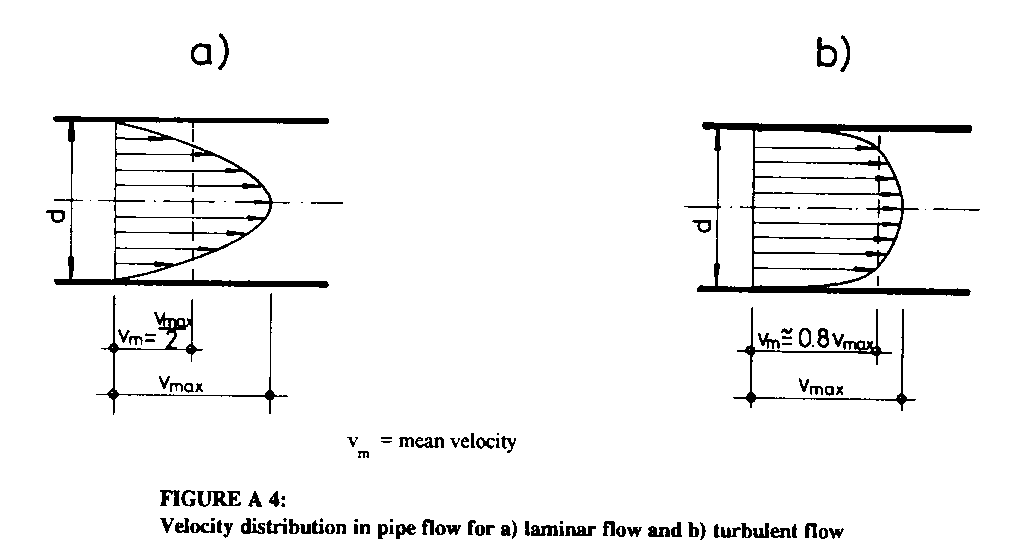
\includegraphics[scale=0.4,natwidth=1024,natheight=554]{laminarpipe} \\ \tiny{\citep[Fig A4]{cef92}} \\ \normalsize
Despite incompressibility and low Reynolds number, the velocity distribution is parabolic. This is due to a boundary condition called the \textbf{kinematic boundary condition}. In words, the boundary condition is simply that particles on the boundary remain there under the image of the flow. This boundary condition is reasonable for `nice' flows (namely homeomorphic flows, as shown in the appendix), but doesn't hold for discontinuous flows.

As we increase the Reynolds number, the laminar idealization breaks down and turbulence begins to take place near the boundaries of the pipe. Part b) of the above image shows turbulent pipe flow.

Next we change the structure of the pipe. The \textbf{partitioned pipe mixer} is constructed by the following procedure: place a plate of length $L$ in the pipe so it divides the flow into 2 semicircles. Place another plate of length $L$ in the pipe orthogonal to the first. Continue this process, alternating the orientation of each plate. 

To analyze the flow in the partitioned pipe mixer, we define the \textbf{mixing strength} as a dimensionless number given by $\beta \approx \frac{4v_RL}{3v_zR}$ \citep[p.~225]{o81}. If $v_R \approx 0$, then negligible mixing will occur since this situation will pertain to regular pressure-driven flow in a semi-circular duct. $\beta$ is intended to be a measure of the cross-sectional stretching per element; the smaller it is, the less mixing occurs.\\ \\
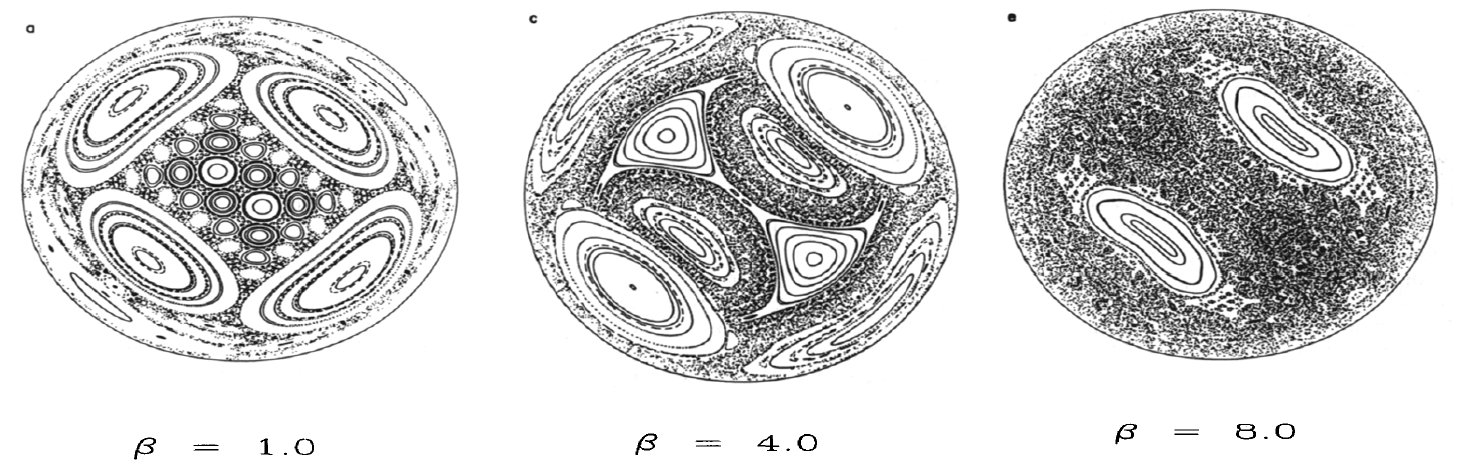
\includegraphics[scale = 0.31, natwidth = 1458, natheight = 472]{poincarebetas}\\ \tiny{\citep[Fig. 5]{kfo87} Poincar\'{e} sections of the partitioned-pipe mixer after 300 iterations with 3 different values of mixing strength $\beta$} \normalsize \\ 
Although the particle paths are continuous, the plates cause discontinuities in the velocities of the fluid, and since the stresses are proportional to the velocity gradient for an incompressible fluid, the stresses here are infinite \citep[~p.227]{o81}. 

Note the presence of KAM tori in the above image, which here look like islands. As mentioned previously, these KAM tori indicate that SMTM is not possible for these flows regardless of how many iterations are done. However it is clear that as beta increases the size and number of KAM tori decrease, indicating a better mix. Also of interest is that the smaller islands actually have higher periods \citep[~p.235]{o81}. 

All of these complications came from splitting the flow repeatedly. Vorticity was created in this process, creating a net rotation for every element of the pipe. 

A further complication can be made. Replace the orthogonal plates with helices of alternating orientation. The image on the following page is for the Kenics$^\copyright$ static mixer.

 If the helices of this mixer are given the same handedness (rather than alternating), the flow is dual to the flow of the partitioned-pipe mixer. This is the same set-up as case B above (RR means right-right). The number immediately following the handedness indicates the angle of the helix (here either 180 or 120 degrees). \\
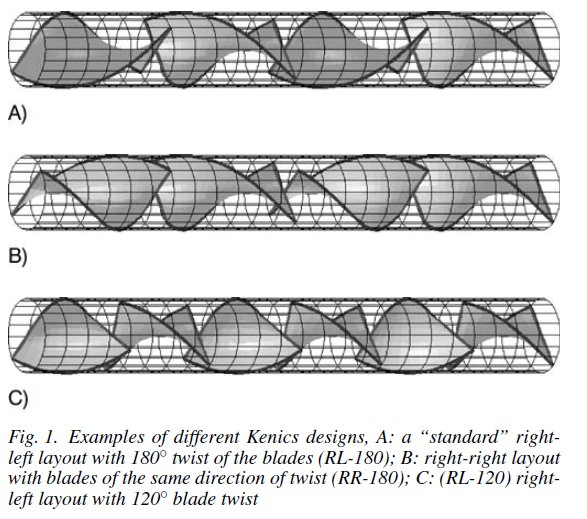
\includegraphics[scale=0.50, natwidth=587, natheight=519]{Kenics}\\ \tiny{\citep[Fig. 1]{getal03}}\\ \normalsize \\
The flow looks like this:\\ \\
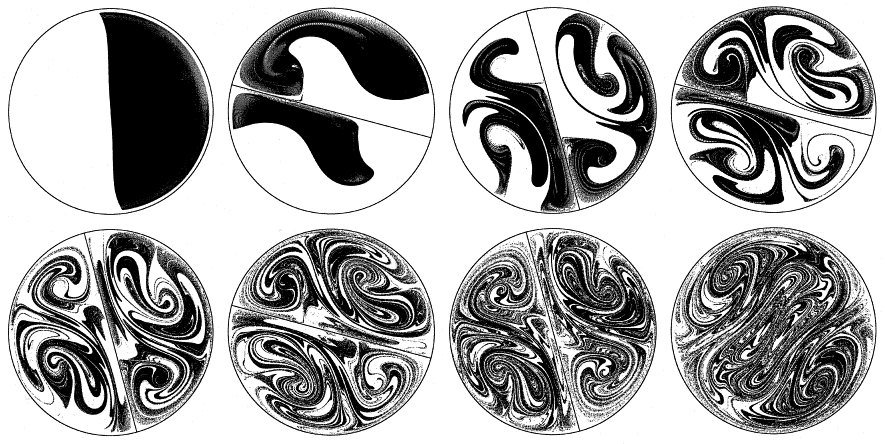
\includegraphics[scale=0.50, natwidth=885, natheight=444]{partpipemixer}\\\tiny{\citep[Fig. 6]{bs99}}\\ \normalsize
\\ \\
Alternating the direction of rotation in the pipe does improve the homogeneity of the flow. That being said, the Kenics$^\copyright$ mixer is still a homeomorphic flow field, and so does not have the cutting necessary for SMTM.  

Stretching, folding, vorticity, and decreasing length scales are all apparent in these examples of pipe flow, and all serve to improve the quality of mixing. 
%%%%%%%%%%%%%%%%%%%%%%%%%%%%%%%%%%%%%%%%%%%%%%%%%%%%%%%%%%%%%%%%%%%%%%%%%%%%%%%%%%%%%%%%%%%%%%%%%%%%%%%%%%%%%%%%%%%%%%%%%%%%%%%%%%%%%%%%%%%%%%%%%%%
\newpage
\section{Appendix}
\subsection{Problem 2.2.2. of Ottino, 1981}

Let $\vec{\Phi}_t(\vec{X})$ be a one parameter family of n-diffeomorphisms which describe the flow of the fluid, such that
\begin{align*}
\{\vec{\Phi}_t(\vec{X}) : \mathbb{R} \times \mathbb{R}^n \mapsto \mathbb{R}^n\;\;\text{ and }\;\; \vec{x} = \vec{\Phi}_t(\vec{X})\}
\end{align*} so $\vec{x}$ is the position of the particle at $\vec{X}$ at time t.$\\ \\$
Let $\{V_0\}$ be a set of n-vectors representing a volume in space containing the collection of particles $\{\vec{X}\}$ at time $t=0$, so $\{V_0\} = \{\vec{X}\}$. Let $\{V_t\} = \{\vec{x}\} =  \vec{\Phi}_t\{V_0\}$ be the volume containing the particles at time t.

\textbf{\citep[Problem 2.2.2.]{o81}}:$\;\;\; \text{Show that }\vec{\Phi}_t\{\partial V_0\} = \{\partial V_t\}\\ \\$
\textbf{Proof}: Consider $\overline{\{V_0\}} = \{V_0\} \cup \{\partial V_0\}$, the closure of $V_0$. Let int$\{V_0\}$ be the interior of $\{V_0\}$.
\begin{align*}
\vec{\Phi}_t\{\text{int}\{V_0\}\}&\subseteq \text{int}\{V_t\}\;\;\;\;\;\;\;\text{because the image of an open set is open under homeomorphisms}\\
\vec{\Phi}_t^{-1}\{\text{int}\{V_t\}\}&\subseteq \text{int}\{V_0\} \;\;\;\;\;\;\;\;\;\;\;\;\;\;\text{(1) because the above holds for preimages too}\\
\text{int}\{V_0\} &= \vec{\Phi}_t^{-1}\{\vec{\Phi}_t\{\text{int}\{V_0\}\}\}\\
&\subseteq \{\vec{\Phi}_t\}^{-1}\{\text{int}\{V_t\}\} \\
&\subseteq \{\text{int}\{V_0\}\}\;\;\;\;\;\;\;\;\;\;\;\;\;\; \text{by (1) }\\
\therefore &\text{the above containments were actually equalities.}\\
\implies \vec{\Phi}_t\{\text{int}\{V_0\}\} &= \text{int}\{V_t\}
\end{align*}
\begin{align*}
&\text{Now we can repeat the procedure using the closures rather than}\\
&\text{ the interiors, and reversing the containments}\\
&\therefore \vec{\Phi}_t\{\overline{\{V_0\}}\} = \overline{\{V_t\}}
\end{align*} Now because $\vec{\Phi}_t$ is bijective, and we now know that it maps the interior to the interior and the closure to the closure, it follows that it maps the boundary to the boundary:
\begin{align*}
\vec{\Phi}_t\{\partial V_0\} &= \vec{\Phi}_t \{\overline{\{V_0\}}\setminus \text{int}\{V_0\}\}\\
&= \overline{\{V_t\}}\setminus\text{int}\{V_t\}\\
&= \{\partial V_t\}
\end{align*}

\newpage
\bibliographystyle{plainnat}
\bibliography{bibliography}
\end{document}o
